\section{Libraries for Data Analysis}
\subsection{Working with Excel}
\subsubsection{Basic Pandas}
Im folgenden werden zwei Pakete benötigt: \textit{Pandas} und \textit{openpyxl}. \\
\begin{lstlisting}[style=python]
	import pandas as pd
	form openpyxl.workbook import Workbook
\end{lstlisting}
Panda ist ein freie Daten Analyse Bibliothek. Bei \textit{openpyxl} handelt es sich um eine Bibiliothek, welche das Lesen und Schreiben von Excel Dateien ermöglicht.\\

Pandas nutzt die folgenden Konzepte um Daten zu speichern und zu manipulieren:
\begin{description}
	\item[Dataframe] Dies wird genutzt, um 2D Tabellen abzuspeichern. 
	\item[Series] Dieses wird genutzt, um 1D Arrays abzuspeichern.
	\item[Panals] Diese wird genutzt, um 3D Daten abzuspeichern.
\end{description}

\paragraph*{pd.read()}
Die Funktion \textit{.read} importiert Daten in den Dataframe. Für verschiedenen Dateiformate bietet Panda unterschiedliche \textit{.read} Funktionen an:
\begin{figure}[H]
	\centering
	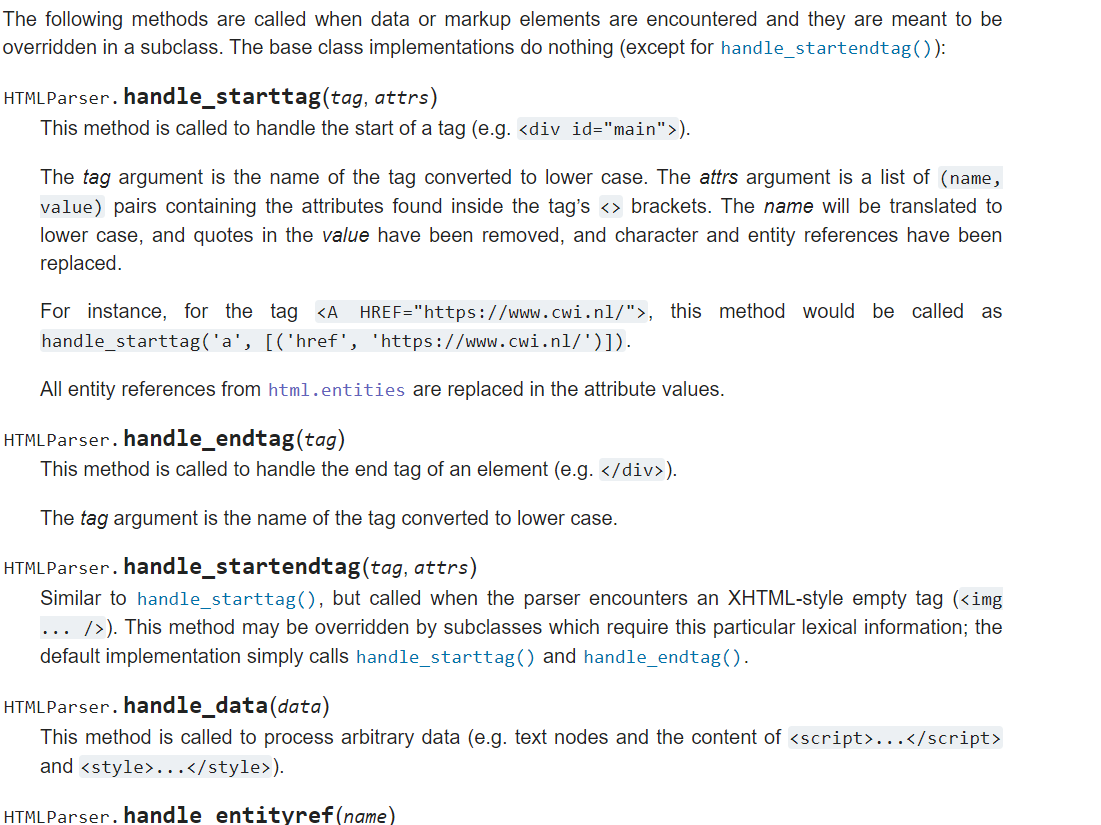
\includegraphics[scale = 0.3]{attachment/chapter_3/Scc077}
\end{figure} 

Das Paket \textit{xlrd} wird benötigt, um die \gls{xlsx} Formate einzulesen. Alternativ kann auch \textit{openpyxl} verwendet werden, um die Dateien einzulesen.
\begin{lstlisting}[style=python]
	# Import Data to Dataframe
	df_excel = pd.read_excel("regions.xlsx",engine='openpyxl')
	# The engine openpyxl was manuell added and installed. Also the Package xlrd was installed in iOS.
	df_csv = pd.read_csv("Names.csv")
	df_text = pd.read_csv("data.txt", delimiter="\t")
\end{lstlisting}

Beim Darstellen der Inhalte werden die ersten fünf und letzten fünf Zeilen ausgewiesen.
\begin{lstlisting}[style=python]
	#                ID  EGF_Baseline  EGF_Stimulus
	#0      FBgn0029994         -1.25         -0.27
	#1      FBgn0037191         -1.05          0.78
	#2      FBgn0036810          2.08          1.34
	#3      FBgn0033320          1.15          0.45
	#4      FBgn0051156         -1.77         -0.76
	#...            ...           ...           ...
	#11761  FBgn0026136          0.57          1.23
	#11762  FBgn0037356          1.14         -0.95
	#11763  FBgn0038214         -1.86         -0.67
	#11764  FBgn0042110          1.49          0.43
	#11765  FBgn0034202         -1.32         -0.22
\end{lstlisting}

In \gls{ETL} Prozess einer \gls{csv} Datei kann wie folgt aussehen.
\begin{lstlisting}[style=python]
	# Extract, Transform and Load
	df_csv = pd.read_csv("Names.csv",header=None)
	df_csv.columns = ["Vorname", "Nachname", "Street", "City", "State", "Postcode", "Unkown"] # Has to be complete.
	df_csv.to_excel("modified.xlsx") # same directory
\end{lstlisting}

\paragraph*{Lambda Function}
Lambda ist eine Funktion, welche zu einer anonymen Funktion referiert.
\begin{align}
	\text{Lambda (Argumgents)}:\text{expression}
\end{align}
Für weiteres siehe iloc Lambda Function. 

\paragraph*{set index}
Mit der Index Funktion kann eine oder mehrere Spalten als Index ausgewählt werden. Ebenso kann verifiziert werden, ob es sich um einen eindeutigen Schlüssel handelt oder nicht.
\begin{lstlisting}[style=python]
	df_new = df_csv.set_index("State", verify_integrity=True)
	### Output
	print(df_new)
	# ValueError: Index has duplicate keys: Index(['NJ', 'SD'], dtype='object', name='State')
\end{lstlisting}
Ohne diese Einschränkung und mit einer anderen Indexspalte wird folgendes wiedergegeben.
\begin{lstlisting}[style=python]
	df_new = df_csv.set_index("Postcode")
	### Output
	print(df_new)
	#
	#                      Vorname  Nachname                            Street         City State  Income
	#Postcode
	#8074                     John       Doe                 120 jefferson st.    Riverside    NJ   45000
	#9119                     Jack  McGinnis                      220 hobo Av.        Phila    PA   18000
	#8075            John "Da Man"    Repici                 120 Jefferson St.    Riverside    NJ  120000
	#91234                 Stephen     Tyler  7452 Terrace "At the Plaza" road     SomeTown    SD   90000
	#298                       NaN  Blankman                               NaN     SomeTown    SD   30000
	#123       Joan "Danger", Anne       Jet               9th, at Terrace plc  Desert City    CO   68000
\end{lstlisting}
\paragraph*{str.split}
Die Splitfunktion zerlegt eine Spalte in ihre Komponenten.
Mit der expand Option wird jede benötigte Abtrennung dargestellt.
\begin{lstlisting}[style=python]
	df_new = df_csv.set_index("Postcode")
	df_new = df_new["Vorname"].str.split(expand=True)
	#df_new = df_new.Vorname.str.split(expand=True) # Same Result
	### Output
	print(df_new)
	#                0          1     2
	#Postcode
	#8074         John       None  None
	#9119         Jack       None  None
	#8075         John        "Da  Man"
	#91234     Stephen       None  None
	#298           NaN        NaN   NaN
	#123          Joan  "Danger",  Anne
\end{lstlisting}
Die erste Spalte wird übertragen, wenn dieser direkt einer andern Spalte zugewiesen wird.
\begin{lstlisting}[style=python]
	df_new = df_csv.set_index("Postcode")
	df_new.Vorname = df_new["Vorname"].str.split(expand=True)
	### Output
	print(df_new)
	#          Vorname  Nachname                            Street         City State  Income
	#Postcode
	#8074         John       Doe                 120 jefferson st.    Riverside    NJ   45000
	#9119         Jack  McGinnis                      220 hobo Av.        Phila    PA   18000
	#8075         John    Repici                 120 Jefferson St.    Riverside    NJ  120000
	#91234     Stephen     Tyler  7452 Terrace "At the Plaza" road     SomeTown    SD   90000
	#298           NaN  Blankman                               NaN     SomeTown    SD   30000
	#123          Joan       Jet               9th, at Terrace plc  Desert City    CO   68000
\end{lstlisting}

\paragraph*{.replace}
Mit der replace Funktion wird ein Wert durch einen anderen Wert ersetzt. Die Konstante np.nan (Convert a string or number to a floating point number, if possible.) gibt Wahr oder Falsch wieder, wenn ein leerer Eintrag existiert.

\begin{lstlisting}[style=python]
	df_new = df_csv.set_index("Postcode")
	df_new.Vorname = df_new["Vorname"].str.split(expand=True)
	df_new = df_new.replace(np.nan, "NaN")
\end{lstlisting}
\subsubsection{Dataframe Functions}
Anhand des Beispiel \textit{Names.csv}.
\begin{lstlisting}[style=python]
	#	               Vorname  Nachname                            Street         City State  Postcode  Unkown
	#	0                 John       Doe                 120 jefferson st.    Riverside    NJ      8074   45000
	#	1                 Jack  McGinnis                      220 hobo Av.        Phila    PA      9119   18000
	#	2        John "Da Man"    Repici                 120 Jefferson St.    Riverside    NJ      8075  120000
	#	3              Stephen     Tyler  7452 Terrace "At the Plaza" road     SomeTown    SD     91234   90000
	#	4                  NaN  Blankman                               NaN     SomeTown    SD       298   30000
	#	5  Joan "Danger", Anne       Jet               9th, at Terrace plc  Desert City    CO       123   68000
\end{lstlisting}
\paragraph{Basics}


\paragraph*{.columns()} weißt den Spalten neue Bezeichnungen zu.
\paragraph*{df.[]} selektiert ausgewählte Spalte, z. B.: .["Vorname"] aus.. Mit einem Array an Spalten [["Vorname"],["Nachname"]] werden mehrere Spalten ausgelesen. Wenn keine Spalte vorliegt, wird diese erzeugt, wenn ihr ein Wert zugewiesen wird. (.["Test"]="Test")

\paragraph*{df.[][]} selektiert im ersten Bereich die Spalte und im zweiten Bereich die Zeilen.
\paragraph*{df.index} Ließt die Index Vektor aus.
\paragraph*{df.drop()} Spalten können entfernt werden. Der Parameter \textit{inplace} gleich \textit{false} gibt, an ob eine Kopie erstellt werden soll. Wird daraufhin \textit{.print()} angewandt, wird der Dataframe ohne die Spalten angezeigt. Wird der Parameter auf \textit{true} gesetzt, so werden die Daten gelöscht.
\begin{lstlisting}[style=python]
	# Drop
	df_new = df_csv.drop(columns=["Postcode"])
	df_new = df_new.groupby(["State"]).mean()
	#Income
	#State        
	# NJ     82500
	# PA     18000
	# SD     30000
	#CO      68000
	#SD      90000
	#>>> 
\end{lstlisting}

\paragraph*{df.head()} Shows a preview

\paragraph*{df.groupby()} Die Spalte, welche gruppiert werden soll, wird hier angegeben. 
\begin{lstlisting}[style=python]
	### Group by
	df_names_modifierd = df_names_modifierd.groupby(["State"]) 
	# Object at 0x...
\end{lstlisting}
Ohne eine spezielle Operation bleibt es bei einem Objekt. Wird die Funktion \textit{.mean()} hinzugefügt, wird diese auf jede Spalte mit Integer angewendet.
\begin{lstlisting}[style=python]
	### Group by
	df_names_modifierd = df_names_modifierd.groupby(["State"]).mean()
	#	       Postcode   Income  Tax Percentage  Tax Amount
	#	State
	#	NJ      8074.5  82500.0            0.25     15000.0
	#	PA      9119.0  18000.0            0.25         0.0
	#	SD       298.0  30000.0            0.25         0.0
	#	CO        123.0  68000.0            0.25     17000.0
	#	SD      91234.0  90000.0            0.25     22500.0
\end{lstlisting}

\paragraph*{df.groupby().mean()} berechnet den Durchschnitt einer Spalte.
\begin{lstlisting}[style=python]
	### Group by
	df_names_modifierd = df_names_modifierd.groupby(["State"]).mean().sort_values("Tax Amount")		
	#       Postcode   Income  Tax Percentage  Tax Amount
	#	State
	#	PA      9119.0  18000.0            0.25         0.0
	#	SD       298.0  30000.0            0.25         0.0
	#	NJ      8074.5  82500.0            0.25     15000.0
	#	CO        123.0  68000.0            0.25     17000.0
	#	SD      91234.0  90000.0            0.25     22500.0
\end{lstlisting}
Wie oben gezeigt, kann die Spalte [Postcode] auch entfernt werden.

\paragraph*{df.apply}
Apply() bietet an, dass Funktionen auf den Dataframe angewandt werden. Diese können weiter auf Bereiche (Achsen) spezifiziert werden.
Mit der Lambda Funktion kann eine Funktion für jeden Eintrag definiert werden. Dabei ist eine genauer Definition nach den Achsen nicht relevant.
\begin{lstlisting}[style=python]
	mydict = [{'a': 1, 'b': 2, 'c': 3, 'd': 4},
	{'a': 100, 'b': 200, 'c': 300, 'd': 400},          
	{'a': 1000, 'b': 2000, 'c': 3000, 'd': 4000 }]
	df_num = pd.DataFrame(mydict)
	
	# Select
	df_new = df_num.apply(lambda x: x+2)
	#df_new = df_num.apply(lambda x: x + 2, axis=0) # Same Result
	#df_new = df_num.apply(lambda x: x + 2, axis=1) # Same Result
	
	# Output
	print(df_new)
	#      a     b     c     d
	#0     3     4     5     6
	#1   102   202   302   402
	#2  1002  2002  3002  4002
	#>>> 
\end{lstlisting}
Mit \textit{axis} 0 oder 1 wird die Funktion entlang der Spalten oder Zeilen durchgeführt. Dies
Mit 0 wird der definierte Funktionsausdruck entlang aller Zeile für jede Spalte durchgeführt. Mit 1 wird für jede Zeile über alle Spalten gerechnet.\\
Für eine Auswahl an Funktion kann das Paket \textbf{numpy} geladen werden.\\

Aggrationen können entlang einer Achse durchgeführt werden. Zurückgegeben wird ein Array. Als default wird die Achse 0 ausgewählt.
\begin{lstlisting}[style=python]
	# Select
	df_new = df_num.apply(np.sum)
	### Output
	print(df_new)
	#a    1101
	#b    2202
	#c    3303
	#d    4404
\end{lstlisting}

Soll entlang einer Zeile die Funktion angewandt werden, wird Achse 1 ausgewählt.
\begin{lstlisting}[style=python]
	# Select
	df_new = df_num.apply(np.sum, axis=1)
	### Output
	print(df_new)
	#0       10
	#1     1000
	#2    10000
\end{lstlisting}

Um Berechnungen an bestimmten Spalten durchzuführen, werden diese an an neue übergeben.
\begin{lstlisting}[style=python]
	# Select
	df_csv["Tax Percentage"] = df_csv["Income"].apply(lambda x: .15 if 0 < x < 10000 else .30 if 10000 <= x < 30000 else .45)
	# if-then-else in one line has change to value_when_true if condition else value_when_false
	df_new = df_csv
	### Output
	print(df_new)
	#               Vorname  Nachname                            Street         City State  Postcode  Income  Tax Percentage
	#0                 John       Doe                 120 jefferson st.    Riverside    NJ      8074   45000            0.45
	#1                 Jack  McGinnis                      220 hobo Av.        Phila    PA      9119   18000            0.30
	#2        John "Da Man"    Repici                 120 Jefferson St.    Riverside    NJ      8075  120000            0.45
	#3              Stephen     Tyler  7452 Terrace "At the Plaza" road     SomeTown    SD     91234   90000            0.45
	#5  Joan "Danger", Anne       Jet               9th, at Terrace plc  Desert City    CO       123   68000            0.45
\end{lstlisting}

Eine Berechnung von zwei Spalten wird durch direktes Aufrufen durchgeführt.
\begin{lstlisting}[style=python]
	# Select
	df_csv["Tax Percentage"] = df_csv["Income"].apply(lambda x: .15 if 0 < x < 10000 else .30 if 10000 <= x < 30000 else .45)
	df_csv["Tax Amount"] = df_csv["Tax Percentage"]*df_csv["Income"]
	df_new = df_csv
	### Output
	print(df_new)
	#               Vorname  Nachname                            Street         City State  Postcode  Income  Tax Percentage  Tax Amount
	#0                 John       Doe                 120 jefferson st.    Riverside    NJ      8074   45000            0.45     20250.0
	#1                 Jack  McGinnis                      220 hobo Av.        Phila    PA      9119   18000            0.30      5400.0
	#2        John "Da Man"    Repici                 120 Jefferson St.    Riverside    NJ      8075  120000            0.45     54000.0
	#3              Stephen     Tyler  7452 Terrace "At the Plaza" road     SomeTown    SD     91234   90000            0.45     40500.0
	#4                  NaN  Blankman                               NaN     SomeTown    SD       298   30000            0.45     13500.0
	#5  Joan "Danger", Anne       Jet               9th, at Terrace plc  Desert City    CO       123   68000            0.45     30600.0
\end{lstlisting}

\paragraph{iloc - Index Number Locator}
Die Methode \textit{iloc[]} oder kurz loc filtert einen Datensatz nach Zeilen und Spalten. Dies Auswahl kann jedoch nur über den jeweiligen zu adressierten Index passieren. Die Berechnungszeit für iloc ist schneller als für loc, genau aus dem Grund, dass die Zeilen und Spalten schon geordnet sind, und somit leichter zu durchsuchen sind.
\paragraph*{Slicer Object} 
Im ersten Beispiel werden alle Zeilen (erste Eingabe vor dem Komma) ausgewählt. Der zweite Eintrag gibt die an, dass alle Spalten bis zur ersten ausgewählt werden sollen. Damit werden beide Achsen gefiltert.
\begin{lstlisting}[style=python]
	df_new = df_csv.iloc[:,:1]
	print(df_new)
	### Output
	#	               Vorname
	#0                 John
	#1                 Jack
	#2        John "Da Man"
	#3              Stephen
	#4                  NaN
	#5  Joan "Danger", Anne
	#>>> 	
\end{lstlisting}

Mit der Änderung auf 3 werden alle Spalten bis einschließlich der dritten Spalte gefiltert.
\begin{lstlisting}
	df_new = df_csv.iloc[:,:3]
	print(df_new)
	### Output
	#	               Vorname  ...                            Street
	#0                 John  ...                 120 jefferson st.
	#1                 Jack  ...                      220 hobo Av.
	#2        John "Da Man"  ...                 120 Jefferson St.
	#3              Stephen  ...  7452 Terrace "At the Plaza" road
	#4                  NaN  ...                               NaN
	#5  Joan "Danger", Anne  ...               9th, at Terrace plc
	#
	#[6 rows x 3 columns]
	#>>> 
\end{lstlisting}
Das Slicer Object kann auch mit einem booleschen Array kombiniert werden. Die Länge des Arrays muss gleich der Länge der zweiten Achse sein.
\begin{lstlisting}[style=python]
	# Select 
	df_new = df_csv.iloc[:,[True, False, False,False,False,False,False]]
	#   Nachname             Street
	#0       Doe  120 jefferson st.
	#1  McGinnis       220 hobo Av.
\end{lstlisting}
Ebenso kann auch eine leere Lambda Funktion oder ein Array für die zweite Achse eingelesen werden.
\begin{lstlisting}[style=python]
	# Select 
	df_new = df_csv.iloc[:, [0, 2]]
	# df_new = df_csv.iloc[:, lambda x: [0,2]] # Same result
	print(df_new)
	### Output
	#               Vorname                            Street
	#0                 John                 120 jefferson st.
	#1                 Jack                      220 hobo Av.
	#2        John "Da Man"                 120 Jefferson St.
	#3              Stephen  7452 Terrace "At the Plaza" road
	#4                  NaN                               NaN
	#5  Joan "Danger", Anne               9th, at Terrace plc
\end{lstlisting}

\paragraph*{Scalar}
Wird Scaler als Eingabe übergeben, wird eine \textit{Series} wiedergegeben und nach Zeilen gefiltert.
\begin{lstlisting}[style=python]
	df_new = df_csv.iloc[1]
	print(df_new)
	### Output
	#
	#Vorname             Jack
	#Nachname        McGinnis
	#Street      220 hobo Av.
	#City               Phila
	#State                 PA
	#Postcode            9119
	#Income             18000
	#Name: 1, dtype: object
	#>>> 
\end{lstlisting}
Mit einem \textbf{zweiten Scaler} wird die Spalte (Achse) ausgewählt. Der Eintrag der Zelle wird wiedergegeben.
\begin{lstlisting}
	df_new = df_csv.loc[1,1] # Zeilen Index 1 (Zweite Zeile), Spalten Index 1 (Zweite Zeile)
	print(df_new)
	#McGinnis
\end{lstlisting}

\paragraph*{Booelen Array}
Wird eine logische Operation (==, <, >) auf eine bestimmt Spalte des Dataframes angewendet, so wird eine \textit{Series} zurückgegeben. Die Series hat die gleiche Länge wie die Tabelle selbst. 
\begin{lstlisting}[style=python]
	# Select 
	df_new = df_csv["State"]=="SD"
	print(df_new)
	### Output
	0    False
	1    False
	2    False
	3     True
	4    False
	5    False
	Name: State, dtype: bool
\end{lstlisting}

Damit die Abfrage genutzt werden kann, muss aus der Serie das Array ausgelesen werden.
\begin{lstlisting}[style=python]
	# Select
	ser_new = df_csv.["State"]=="SD"
	#df_new = df_csv.loc[ser_new]
	print(df_new)
	### Output
	#   Vorname Nachname                            Street      City State  Postcode  Income
	#3  Stephen    Tyler  7452 Terrace "At the Plaza" road  SomeTown    SD     91234   90000
	#4      NaN  Blankman                               NaN  SomeTown    SD       298   30000
\end{lstlisting}
Mit iloc kann nur ein Array von Boolschen Werten eingelesen werden. Dies Serie muss nur nach dem Array ausgewertet werden.
\begin{lstlisting}[style=python]
	# Select
	ser_new = df_csv.["State"]=="SD"
	#df_new = df_csv.iloc[ser_new.array] # Array gibt ein narray wieder.
	print(df_new)
	### Output
	#   Vorname Nachname                            Street      City State  Postcode  Income
	#3  Stephen    Tyler  7452 Terrace "At the Plaza" road  SomeTown    SD     91234   90000
	#4      NaN  Blankman                               NaN  SomeTown    SD       298   30000
\end{lstlisting}
Alternativ muss ein Array der Länge des Dataframes eingegeben werde.
\begin{lstlisting}[style=python]                          NaN  SomeTown    SD       298   30000
	# Select 
	df_new = df_csv.loc[[False,False,False,True,False,False]]
	#df_new = df_csv.iloc[[False,False,False,True,False,False]] # loc bietet die gleiche Eingabemöglichkeit
	print(df_new)
	### Output
	#   Vorname Nachname                            Street      City State  Postcode  Income
	#3  Stephen    Tyler  7452 Terrace "At the Plaza" road  SomeTown    SD     91234   90000
	#4      NaN  Blankman                               NaN  SomeTown    SD       298   30000
\end{lstlisting}

\paragraph*{List of Integers(Index)}
Über iloc können auch die Indizes direkt eingegeben werden. Dafür werden sie als Array eingespielt.
\begin{lstlisting}[style=python]
	# Select
	df_new = df_csv.iloc[[0,1,2]]
	print(df_new)
	### Output
	#      	 Vorname  Nachname             Street       City State  Postcode  Income
	#0           John       Doe  120 jefferson st.  Riverside    NJ      8074   45000
	#1           Jack  McGinnis       220 hobo Av.      Phila    PA      9119   18000
	#2  John "Da Man"    Repici  120 Jefferson St.  Riverside    NJ      8075  120000
\end{lstlisting}
Mit dem zweiten Eintrag wird die zweite Achse gefiltert.
\begin{lstlisting}[style=python]
	# Select
	df_new = df_csv.iloc[[0,1,2],[1,2]]
	print(df_new)
	### Output
	#   Nachname             Street
	#0       Doe  120 jefferson st.
	#1  McGinnis       220 hobo Av.
	#2    Repici  120 Jefferson St.
\end{lstlisting}
\paragraph*{iloc with Lambda Function}
Lambda ist eine Funktion, welche zu einer anonymen Funktion referiert.
\begin{align}
	\text{Lambda (Argumgents)}:\text{expression}
\end{align}
Eine Lambda Funktion kann ebenso mit iloc verwendet werden. Im folgenden Beispiel wird der Ausdruck Modular 2 auf die Indizes der Zeilen angewandt. Das Argument $x$ ist dabei der Dataframe selbst. Mit .index werden die Indizes ausgelesen. Jeder gerade Zeilen Index wird ausgewählt.
\begin{lstlisting}[style=python]
	# Select 
	df_new = df_csv.iloc[lambda x: x.index % 2 == 0]
	print(df_new)
	### Output
	#         Vorname  Nachname             Street       City State  Postcode  Income
	#0           John       Doe  120 jefferson st.  Riverside    NJ      8074   45000
	#2  John "Da Man"    Repici  120 Jefferson St.  Riverside    NJ      8075  120000
	#4            NaN  Blankman                NaN   SomeTown    SD       298   30000
\end{lstlisting}

\paragraph{loc - Index Name Locator}
\paragraph*{Slicer Object, Scalar, List of Name Integers}
Der Fokus der loc Funktion ist, das die Indexes eine String Bezeichnungen besitzen. Im folgenden Beispiel wurden die Indizes für Zeilen und Spalten mit Strings näher definiert.
\begin{lstlisting}[style=python]
	# Select 
	#df_new = df_csv.iloc[:, [0, 2]]
	df = pd.DataFrame([[1, 2], [4, 5], [7, 8]],
	index=['cobra', 'viper', 'sidewinder'],
	columns=['max_speed', 'shield'])
	
	df_new = df.loc["cobra"]
	print(df_new)
	### Output
	#max_speed    1
	#shield       2
	#Name: cobra, dtype: int64
\end{lstlisting}
\begin{lstlisting}[style=python]
	# Select 
	df = pd.DataFrame([[1, 2], [4, 5], [7, 8]],
	index=['cobra', 'viper', 'sidewinder'],
	columns=['max_speed', 'shield'])
	
	df_new = df.loc["cobra","max_speed]
	print(df_new)
	### Output
	#1
\end{lstlisting}
Für den Slicer lässt sich die Logik auch übertragen.
\begin{lstlisting}[style=python]
	# Select 
	df = pd.DataFrame([[1, 2], [4, 5], [7, 8]],
	index=['cobra', 'viper', 'sidewinder'],
	columns=['max_speed', 'shield'])
	
	df_new = df.loc["cobra": "sidewinder"]
	print(df_new)
	### Output
	#            max_speed  shield
	#cobra               1       2
	#viper               4       5
	#sidewinder          7       8
\end{lstlisting}

\paragraph*{Booelen Array/ Series}
Es gilt das gleich wie bei iloc, bis auf die Ergänzung, dass Abfragen mit einem Serie ebenfalls gefüllt werden kann.

\begin{lstlisting}[style=python]
	# Select 
	df_new = df_csv.loc[df_csv["State"]=="SD"]
	#df_new = df_csv.loc[[False,False,False,True,False,False]] # Same Result
	print(df_new)
	### Output
	#   Vorname Nachname                            Street      City State  Postcode  Income
	#3  Stephen    Tyler  7452 Terrace "At the Plaza" road  SomeTown    SD     91234   90000
\end{lstlisting}
Ergänzend kann auch eine bedingte Abfrage mit einer Spaltenauswahl getroffen werden.
\begin{lstlisting}[style=python]
	df = pd.DataFrame([[1, 2], [4, 5], [7, 8]],
	index=['cobra', 'viper', 'sidewinder'],
	columns=['max_speed', 'shield'])
	
	df_new = df.loc[df["max_speed"]>0, ["shield"]]
	print(df_new)
	### Output
	#            shield
	#cobra            2
	#viper            5
	#sidewinder       8
\end{lstlisting}

\paragraph*{Change spezific Values based on condition}
Im Abschnitt df.apply wurden Steuersätze eingefügt. Diese Beispiel soll dienen, wie genau Daten geändert werden.
\begin{lstlisting}[style=python]
	# Select
	df_csv["Tax Percentage"] = df_csv["Income"].apply(lambda x: .15 if 0 < x < 10000 else .30 if 10000 <= x < 30000 else .45)
	df_csv["Tax Amount"] = df_csv["Tax Percentage"]*df_csv["Income"]
	
	df_new = df_csv.drop(columns=["Street","City", "State", "Postcode"])
	df_new.loc[df_new["Tax Percentage"]<= .3, "Tax Amount"] = 0
	### Output
	print(df_new)
	#               Vorname  Nachname  Income  Tax Percentage  Tax Amount
	#0                 John       Doe   45000            0.45     20250.0
	#1                 Jack  McGinnis   18000            0.30         0.0
	#2        John "Da Man"    Repici  120000            0.45     54000.0
	#3              Stephen     Tyler   90000            0.45     40500.0
	#4                  NaN  Blankman   30000            0.45     13500.0
	#5  Joan "Danger", Anne       Jet   68000            0.45     30600.0
\end{lstlisting}


\subsubsection{openpyxl}

\paragraph{Load existing workbook}
Um bestehenden Excel Dokumente zu laden, wird das Paket \textit{load}$\_$\textit{workbook} benötigt.
\begin{lstlisting}[style=python]
	from openpyxl import load_workbook
	
	wb_load = load_workbook("regions.xlsx")
	output = wb_load.sheetnames
	
	# Print
	print(output)
	#['Sheet1']
\end{lstlisting}

\paragraph{Workbook}
Das Paket Workbook bietet die Möglichkeit Workbooks direkt im Arbeitsspeicher zu erstellen, ohne diese vorher gespeichert zu haben.
\begin{lstlisting}[style=python]
	from openpyxl import load_workbook
	from openpyxl import Workbook
	
	wb_load = load_workbook("regions.xlsx")
	
	# Create new Workbook
	wb_new = Workbook()
	
	# Create new Worksheets
	ws1 = wb_new.create_sheet("New Sheet2",1)
	ws0 = wb_new.create_sheet("Legende", 0)
	ws2 = wb_new.create_sheet("Vorletze",-1)
	
	output = wb_new.sheetnames
	
	# Print
	print(output)
	# ['Legende', 'Sheet', 'Vorletze', 'New Sheet2']
\end{lstlisting}
Die Funktion \textit{create}$\_$\textit{sheet} hat als zweiten optionalen Parameter die Reihenfolge definiert. Diese startet bei 0.
Den Titel eines Sheets kann direkt mit \textit{.title} abgefragt werden.

\begin{lstlisting}[style=python]
	print(wb_new["Legende"].title)
	print(ws0.title) 
	#Legende
	#Legende
\end{lstlisting}

Ebenso kann über alle Worksheets interiert werden.
\begin{lstlisting}[style=python]
	for ws in wb_new:
	print(ws.title)
	#Legende
	#Sheet
	#Vorletze
	#New Sheet2
\end{lstlisting}

Ein bestimmtes Worksheet zu bearbeiten, erfordert es das zugehörige Workbook zu aktivieren.
\begin{lstlisting}[style=python]
	wb_new.active
	ws1["A4"] = 4
	output = ws1["A4"].value
	# 4
	wb_new.save("regions_new.xlsx")
\end{lstlisting}

Um das Workbook zu speichern, wird die save() Funktion genannt.

\paragraph{Select}
Zellen, Zeilen und Spalten können direkt über den ausgewählten Sheet angesteuert werden. 
\begin{lstlisting}[style=python]
	#from openpyxl import Workbook
	#import openpyxl as op
	from openpyxl import load_workbook
	from openpyxl import Workbook
	
	wb_load = load_workbook("regions.xlsx")
	
	# Create new Workbook
	wb_new = Workbook()
	
	# Create new Worksheets
	ws1 = wb_new.create_sheet("New Sheet2",1)
	ws0 = wb_new.create_sheet("Legende", 0)
	ws2 = wb_new.create_sheet("Vorletze",-1)
	
	wb_load.active
	
	for i in wb_load:
	print(i.title)
	
	range = wb_load["Sheet1"]["A1": "B7"]
	
	for i in range:
	for j in i:0
	print(j.value)	
\end{lstlisting}

Es gibt ebenso eine Iteration Funktion für Zeilen und Spalten.
\begin{lstlisting}[style=python]
	#from openpyxl import Workbook
	#import openpyxl as op
	from openpyxl import load_workbook
	from openpyxl import Workbook
	
	wb_load = load_workbook("regions.xlsx")
	
	# Create new Workbook
	wb_new = Workbook()
	
	# Create new Worksheets
	ws1 = wb_new.create_sheet("New Sheet2",1)
	ws0 = wb_new.create_sheet("Legende", 0)
	ws2 = wb_new.create_sheet("Vorletze",-1)
	
	ws = wb_load.active
	
	for i in wb_load:
	print(i.title)
	
	range = ws.iter_rows(min_row = 1, max_row = 3, max_col = 3, values_only = True)
	
	for i in range:
	for j in i:
	print(j)
	### Output
	#Sheet1
	#Region
	#Units
	#Sales
	#South
	#54
	#332
	#North
	#20
	#110
	#>>>
	
	### Output without values_only = True
	#Sheet1
	#<Cell 'Sheet1'.A1>
	#<Cell 'Sheet1'.B1>
	#<Cell 'Sheet1'.C1>
	#<Cell 'Sheet1'.A2>
	#<Cell 'Sheet1'.B2>
	#<Cell 'Sheet1'.C2>
	#<Cell 'Sheet1'.A3>
	#<Cell 'Sheet1'.B3>
	#<Cell 'Sheet1'.C3>
	#>>>  	
\end{lstlisting}

\paragraph{Mutliple Sheets}
Es können mehre Dateien und mehrere Tabellenblätter ausgelesen werden.
\begin{lstlisting}[style= python]
	import pandas as pd
	import time
	start_time = time.time()
	
	# Load data
	df_1 = pd.read_excel("shifts.xlsx", sheet_name= "Sheet1", skiprows=2, engine='openpyxl', usecols=lambda x: 'Unnamed' not in x)
	df_2 = pd.read_excel("shifts.xlsx", sheet_name= "Sheet1", skiprows=2, engine='openpyxl', usecols=lambda x: 'Unnamed' not in x)
	df_3 = pd.read_excel("shift_3.xlsx", skiprows=2, engine='openpyxl', usecols=lambda x: 'Unnamed' not in x)
	
	df_4 = pd.concat([df_1, df_2, df_3])
	
	
	print(df_4)
	print("--- %s seconds ---" % (time.time() - start_time))
	### Output
	#    Shift  ... Units Sold
	#0       2  ...        157
	#1       2  ...         83
	#2       2  ...        180
	#3       2  ...        186
	#4       2  ...        117
	#..    ...  ...        ...
	#94      3  ...         42
	#95      3  ...        168
	#96      3  ...        132
	#97      3  ...        111
	#98      3  ...        151
	#
	#[299 rows x 6 columns]
	#--- 0.4967920780181885 seconds ---
	#>>> 
\end{lstlisting}
\paragraph{Store Data from Dataframe into Workbook}
Mit der Funktion dataframe-to-rows wird ein Dataframe in Zeilen zerlegt. Die Werte aus diesen können einzeln adressiert werden und spezifischen Zellen in einem Worksheet zugewiesen werden.

\subsection{Exploritory Data Analysis}

Das Konzept \gls{EDA} wird unterschiedlich verwendet. Diese dient, die zu verwendenden Daten zu verstehen.

\subsubsection{Overview} 
\begin{itemize}
	\item df.head()
	\item for col in df.columns
	\item df.tail()
	\item df.shape
	\item df.describe()
	\item df[].unique()
	\item df.nunique()
	\item df.drop()
\end{itemize}
Als Datenquelle werden die COVID Zahlen des \gls{RKI} mit \href{https://npgeo-corona-npgeo-de.hub.arcgis.com/datasets/dd4580c810204019a7b8eb3e0b329dd6_0}{Flat-File.}
Die Legende findet sich unter \href{https://npgeo-corona-npgeo-de.hub.arcgis.com/datasets/dd4580c810204019a7b8eb3e0b329dd6_0}{Legende-RKI}
\paragraph{head()}
Im ersten Schritt werden die ersten Zeilen angezeigt.
\begin{lstlisting}[style= python]
	import pandas as pd
	import numpy as np
	import seaborn as sb
	
	df_rki = pd.read_csv("RKI_COVID19.csv")
	
	print(df_rki.head())
	### Output
	#   ObjectId  ...      Altersgruppe2
	#0         1  ...  Nicht übermittelt
	#1         2  ...  Nicht übermittelt
	#2         3  ...  Nicht übermittelt
	#3         4  ...  Nicht übermittelt
	#4         5  ...  Nicht übermittelt
	#
	#[5 rows x 18 columns]
	#>>> 	
\end{lstlisting}
\paragraph{columns}
Die einzelnen Namen der Spalten werden über eine Iteration angezeigt.
\begin{lstlisting}[style=python]
	for col in df_rki.columns:
	print(col)
	### Output
	ObjectId
	IdBundesland
	Bundesland
	Landkreis
	Altersgruppe
	Geschlecht
	AnzahlFall
	AnzahlTodesfall
	Meldedatum
	IdLandkreis
	Datenstand
	NeuerFall
	NeuerTodesfall
	Refdatum
	NeuGenesen
	AnzahlGenesen
	IstErkrankungsbeginn
	Altersgruppe2
	>>> 
	
	# tail() shows the last five entries	
	print(df.tail())
	### Output
	#         ObjectId  ...      Altersgruppe2
	#1134991   1134992  ...  Nicht übermittelt
	#1134992   1134993  ...  Nicht übermittelt
	#1134993   1134994  ...  Nicht übermittelt
	#1134994   1134995  ...  Nicht übermittelt
	#1134995   1134996  ...  Nicht übermittelt
	#
	#[5 rows x 18 columns]
	#>>> 
\end{lstlisting}
\paragraph{describe()}
Die Funktion\textit{describe()} gibt einen Standardabfrage an den Dataframe wieder.
\begin{lstlisting}[style=python]
	df = pd.read_csv("RKI_COVID19.csv")
	df_a = df["Altersgruppe"]
	x = df_a.describe()
	print(x)
	### Output
	#
	#count     1134996
	#unique          7
	#top       A35-A59
	#freq       386139
	#Name: Altersgruppe, dtype: object
	#>>> 
\end{lstlisting}
Als nächstes wird ein Jupyter Auszug einfügt, in welcher weiter mit der describe() Funktion gearbeitet wird.

\begin{figure}[H]
	\centering
	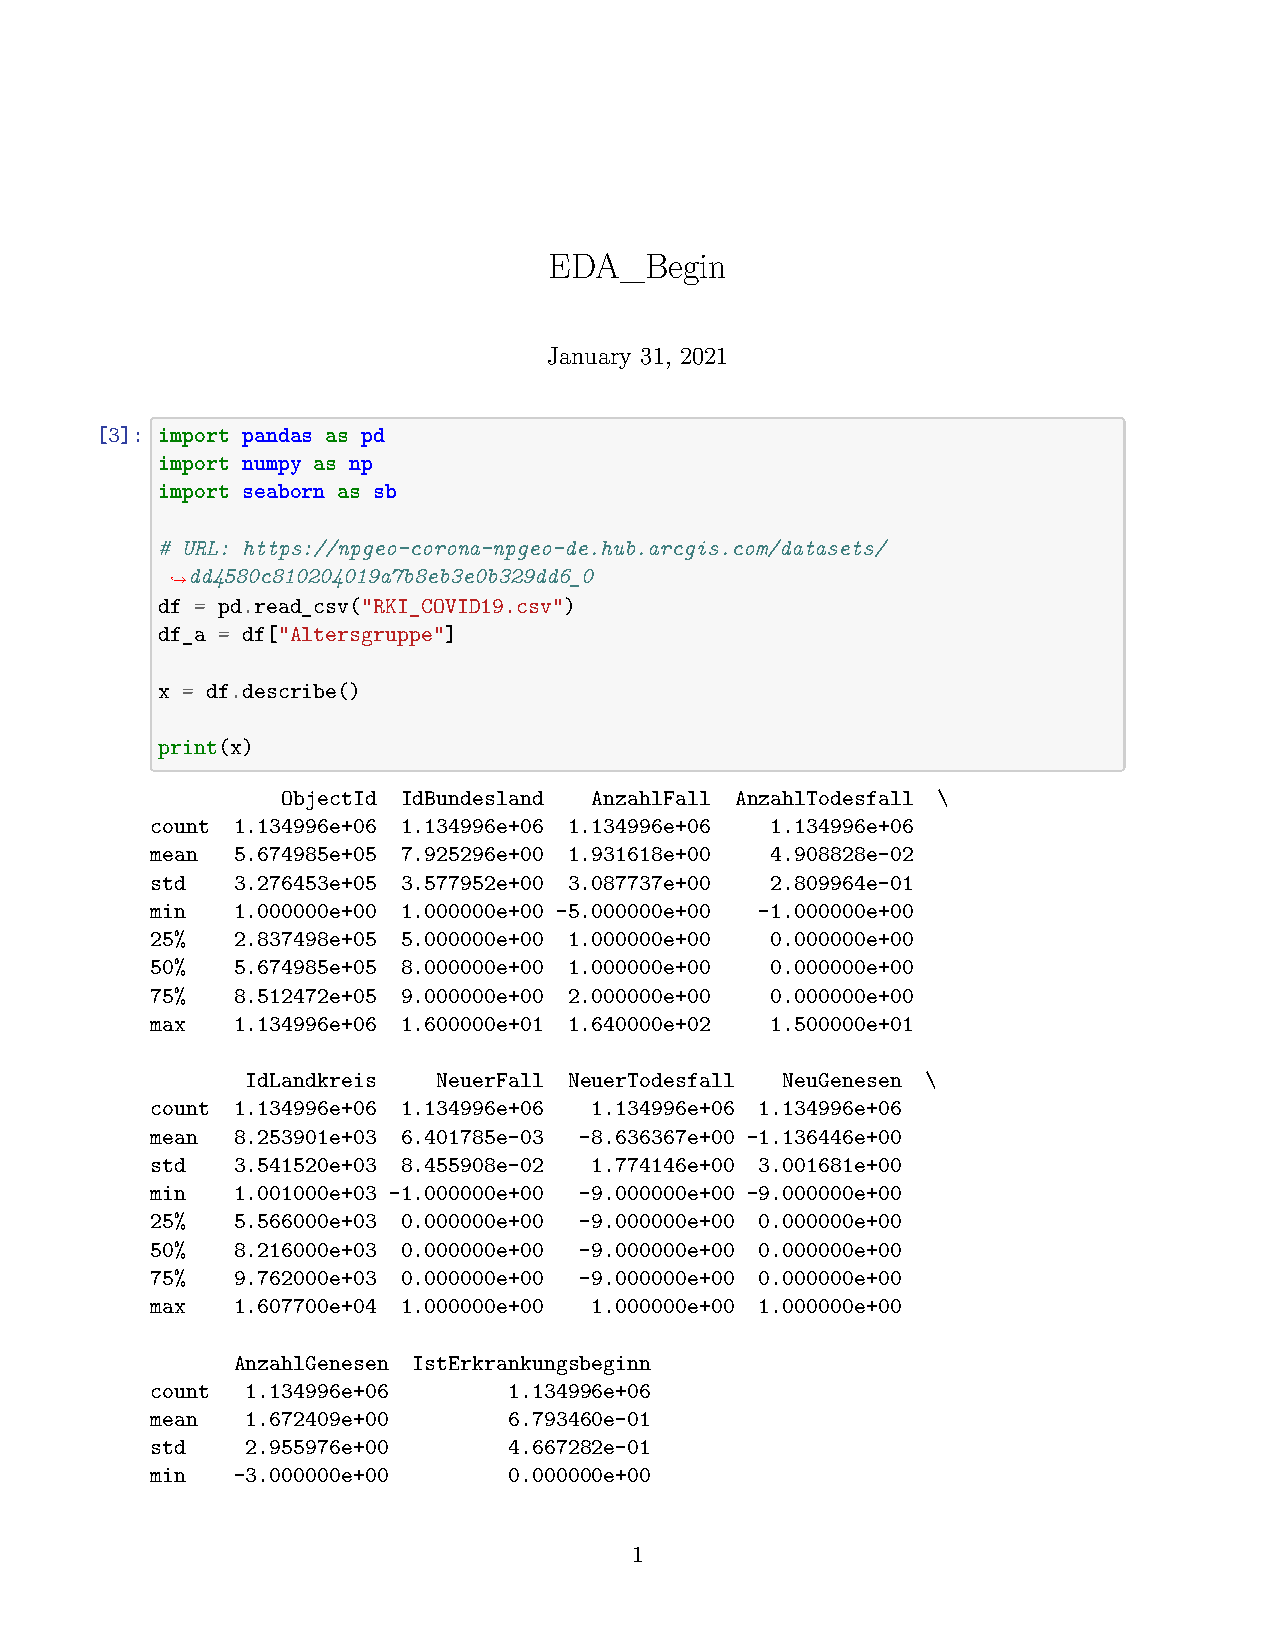
\includegraphics[scale = 0.8]{attachment/chapter_3/Scc078}
\end{figure} 

\paragraph{nunique() unique()}
Mit dieser Funktion werden alle Spalten abgegangen und die verschiedenen Werte wieder gegeben.
\begin{lstlisting}[style=python]
	df.nunique()
	ObjectId                1134996
	IdBundesland                 16
	Bundesland                   16
	Landkreis                   412
	Altersgruppe                  7
	Geschlecht                    3
	AnzahlFall                  128
	AnzahlTodesfall              16
	Meldedatum                  380
	IdLandkreis                 412
	Datenstand                    1
	NeuerFall                     3
	NeuerTodesfall                4
	Refdatum                    394
	NeuGenesen                    4
	AnzahlGenesen               127
	IstErkrankungsbeginn          2
	Altersgruppe2                 1
	dtype: int64
\end{lstlisting}
Sollen die Werte der jeweiligen Spalte ausgegeben werden, so bietet sich die Funktion unique() an.
\begin{lstlisting}[style=python]
	df["Geschlecht"].unique()
	array(['M', 'W', 'unbekannt'], dtype=object)
	df["NeuerFall"].unique()
	array([ 0, -1,  1], dtype=int64)
\end{lstlisting}

\paragraph{Check for Nullvalues}
In zwei Schritte kann eine Übersicht geschaffen werden, welche Ausschluss über die leere Werte im Dataframe gibt.
\begin{lstlisting}[style=python]
	df.isnull().sum()
	ObjectId                0
	IdBundesland            0
	Bundesland              0
	Landkreis               0
	Altersgruppe            0
	Geschlecht              0
	AnzahlFall              0
	AnzahlTodesfall         0
	Meldedatum              0
	IdLandkreis             0
	Datenstand              0
	NeuerFall               0
	NeuerTodesfall          0
	Refdatum                0
	NeuGenesen              0
	AnzahlGenesen           0
	IstErkrankungsbeginn    0
	Altersgruppe2           0
	dtype: int64
\end{lstlisting}
Mit Isnull() wird eine logische Überprüfung durchgeführt werden. Mit der Summe über alle Spalten wird die Menge der leeren Werte summiert angezeigt.

\paragraph{Convert Date as String to Date type}
Die übergebenen Datumswerte sind als String übergeben. Um diese filtern und weiter bearbeiten zu können, werde diese mit dem Paket \textit{datetime} umgewandelt.
\begin{lstlisting}[style=python]
	#%%
	import pandas as pd
	import numpy as np
	import seaborn as sb
	import datetime as dt
	
	# URL: https://npgeo-corona-npgeo-de.hub.arcgis.com/datasets/dd4580c810204019a7b8eb3e0b329dd6_0
	df = pd.read_csv("RKI_COVID19.csv")
	
	df_SKA = df.loc[df["Landkreis"]=="SK Augsburg"]
	df_SKA = df_SKA[["Meldedatum","AnzahlFall"]]
	df_SKA = df_SKA.iloc[0:3]
	df_SKA["Date"] = df_SKA["Meldedatum"].apply(lambda x: dt.datetime.strptime(x, '%Y/%m/%d %H:%M:%S')) # apply 
	df_SKA["year"] = df_SK["Date"].apply(lambda x: x.year)
	df_SKA["Month"] =  df_SKA["Date"].apply(lambda x: x.month)
	df_SKA["Day"] =  df_SKA["Date"].apply(lambda x: x.day)
	df_SKA.drop(["Meldedatum"], axis=1, inplace=True) # inplace modifize the same variable
	df_SKA.head()
	
	# %%
	#AnzahlFall	Date	year	Month	Day
	#845500	1	2020-09-13	2020	9	13
	#845503	1	2020-05-28	2020	5	28
	#845504	1	2020-05-31	2020	5	31
\end{lstlisting}

\paragraph{Histogramm}
Anteil der Infektionen:
\begin{lstlisting}[style=python]
	#%%
	import pandas as pd
	import numpy as np
	import seaborn as sb
	import datetime as dt
	
	# Source
	# URL: https://npgeo-corona-npgeo-de.hub.arcgis.com/datasets/dd4580c810204019a7b8eb3e0b329dd6_0
	df_SKA = pd.read_csv("RKI_COVID19.csv")
	
	#Select Data for Augsburg
	df_SKA = df_SKA.loc[df_SKA["Landkreis"]=="SK Augsburg"]
	
	# Filter for Infected People
	df_SKA = df_SKA.loc[lambda df: (df["AnzahlFall"]>0) & (df["AnzahlTodesfall"]<=0)]
	
	# Drops other columns
	Import_Col = [
	"Meldedatum",
	"AnzahlFall",
	"NeuerFall",
	"AnzahlTodesfall",
	"Altersgruppe"
	]
	df_SKA = df_SKA[Import_Col]
	
	#  Fix Date
	df_SKA["Date"] = df_SKA["Meldedatum"].apply(lambda x: dt.datetime.strptime(x, '%Y/%m/%d %H:%M:%S'))
	df_SKA["year"] = df_SKA["Date"].apply(lambda x: x.year)
	df_SKA["Month"] =  df_SKA["Date"].apply(lambda x: x.month)
	df_SKA["Day"] =  df_SKA["Date"].apply(lambda x: x.day)
	df_SKA.drop(["Meldedatum"], axis=1, inplace=True)
	
	# Sort Values
	df_SKA.sort_values(by=["Date"], inplace=True)
	
	# Show Histogram
	df_SKA["Altersgruppe"].hist()
\end{lstlisting}
\begin{figure}[H]
	\centering
	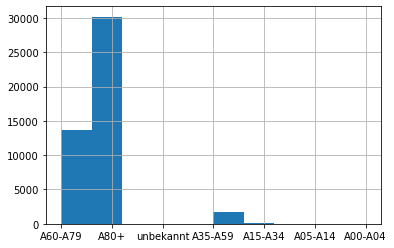
\includegraphics[scale = 0.8]{attachment/chapter_3/Scc082}
\end{figure} 
und der Todesfälle in Deutschland.
\begin{lstlisting}[style=python]
	# Filter for Infected People
	df_SKA = df_SKA.loc[lambda df: (df["AnzahlFall"]>0) & (df["AnzahlTodesfall"]>0)]
\end{lstlisting}
\begin{figure}[H]
	\centering
	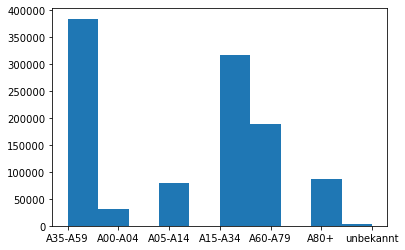
\includegraphics[scale = 0.8]{attachment/chapter_3/Scc083}
\end{figure} 
\subsubsection{Relationship Analysis}
\paragraph{Correlation, Headmap, Correlation}
\begin{itemize}
	\item seaborn df.corr()
	\item sns.headmap(df.corr())
	\item sns.pairplot(df)
\end{itemize}
Beide Funktionen corr() und sns.headmap() können nur auf metrische Variablen angewendet werden.
\begin{lstlisting}[style=python]
	import pandas as pd
	import numpy as np
	import seaborn as sns
	import datetime as dt
	
	from seaborn.palettes import color_palette
	
	# Source
	# URL: https://npgeo-corona-npgeo-de.hub.arcgis.com/datasets/dd4580c810204019a7b8eb3e0b329dd6_0
	df_SKA = pd.read_csv("RKI_COVID19.csv")
	
	#Select Data for Augsburg
	#df_SKA = df_SKA.loc[df_SKA["Landkreis"]=="SK Augsburg"]
	#	ObjectId, 
	#   IdBundesland
	#   Bundesland
	# 	Landkreis
	#   Altersgruppe
	#   Geschlecht
	#	AnzahlFall 
	# 	AnzahlTodesfall
	#	Meldedatum
	#	IdLandkreis
	#	Datenstand
	#	NeuerFall
	#	NeuerTodesfall
	#	Refdatum
	#	NeuGenesen
	#	AnzahlGenesen
	#	IstErkrankungsbeginn
	#	Altersgruppe2
	
	# Filter for Infected People
	df_SKA = df_SKA.loc[lambda df: (df["AnzahlFall"]>0) & (df["AnzahlTodesfall"]>0)]
	
	# Drops other columns
	Import_Col = [
	"Meldedatum",
	"AnzahlFall",
	"AnzahlTodesfall",
	"Altersgruppe",
	#"IdBundesland",
	"IdLandkreis",
	"Geschlecht"
	]
	df_SKA = df_SKA[Import_Col]
	
	#  Fix Date
	df_SKA["Date"] = df_SKA["Meldedatum"].apply(lambda x: dt.datetime.strptime(x, '%Y/%m/%d %H:%M:%S'))
	#df_SKA["year"] = df_SKA["Date"].apply(lambda x: x.year)
	#df_SKA["Month"] =  df_SKA["Date"].apply(lambda x: x.month)
	#df_SKA["Day"] =  df_SKA["Date"].apply(lambda x: x.day)
	df_SKA.drop(["Meldedatum"], axis=1, inplace=True)
	
	# Sort Values
	#df_SKA.sort_values(by=["Date"], inplace=True)
	
	# Relationship
	correlation = df_SKA.corr()
	sns.heatmap(correlation,xticklabels=correlation.columns, yticklabels=correlation.columns, annot=True)
	
	sns.pairplot(df_SKA)
\end{lstlisting}
\begin{figure}[H]
	\centering
	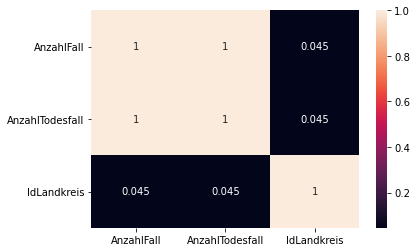
\includegraphics[scale = 0.8]{attachment/chapter_3/Scc081}
\end{figure} 

\begin{figure}[H]
	\centering
	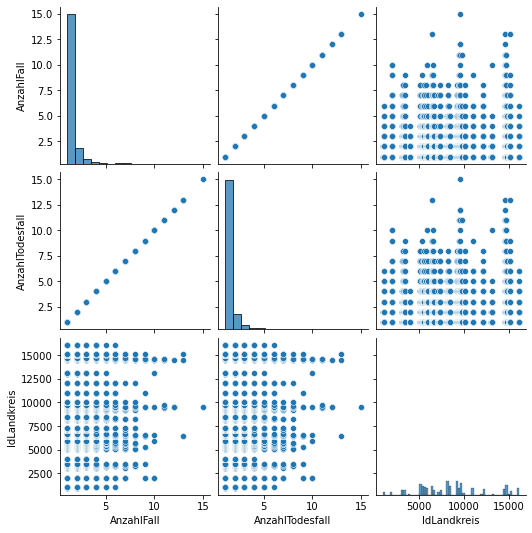
\includegraphics[scale = 0.8]{attachment/chapter_3/Scc080}
\end{figure} 
\paragraph{Relplot for Ordinal Data (Skatter Plot)}
\begin{lstlisting}[style=python]
	#%%
	import pandas as pd
	import numpy as np
	import seaborn as sns
	import datetime as dt
	
	from seaborn.palettes import color_palette
	
	# Source
	# URL: https://npgeo-corona-npgeo-de.hub.arcgis.com/datasets/dd4580c810204019a7b8eb3e0b329dd6_0
	df_SKA = pd.read_csv("RKI_COVID19.csv")
	
	#Select Data for Augsburg
	#df_SKA = df_SKA.loc[df_SKA["Landkreis"]=="SK Augsburg"]
	#	ObjectId, 
	#   IdBundesland
	#   Bundesland
	# 	Landkreis
	#   Altersgruppe
	#   Geschlecht
	#	AnzahlFall 
	# 	AnzahlTodesfall
	#	Meldedatum
	#	IdLandkreis
	#	Datenstand
	#	NeuerFall
	#	NeuerTodesfall
	#	Refdatum
	#	NeuGenesen
	#	AnzahlGenesen
	#	IstErkrankungsbeginn
	#	Altersgruppe2
	
	# Filter for Infected People
	df_SKA = df_SKA.loc[lambda df: (df["AnzahlFall"]>0) & (df["AnzahlTodesfall"]>0)]
	
	# Drops other columns
	Import_Col = [
	"Meldedatum",
	#"AnzahlFall",
	"AnzahlTodesfall",
	"Altersgruppe",
	#"IdBundesland",
	#"IdLandkreis",
	"Geschlecht"
	]
	df_SKA = df_SKA[Import_Col]
	
	#  Fix Date
	df_SKA["Date"] = df_SKA["Meldedatum"].apply(lambda x: dt.datetime.strptime(x, '%Y/%m/%d %H:%M:%S'))
	#df_SKA["year"] = df_SKA["Date"].apply(lambda x: x.year)
	#df_SKA["Month"] =  df_SKA["Date"].apply(lambda x: x.month)
	df_SKA["Day"] =  df_SKA["Date"].apply(lambda x: x.day)
	df_SKA.drop(["Meldedatum"], axis=1, inplace=True)
	
	# Sort Values
	#df_SKA.sort_values(by=["Date"], inplace=True)
	
	# Relationship
	sns.relplot(x= "Date",y="AnzahlTodesfall", hue="Geschlecht", data=df_SKA)
	# %%
\end{lstlisting}
\begin{figure}[H]
	\centering
	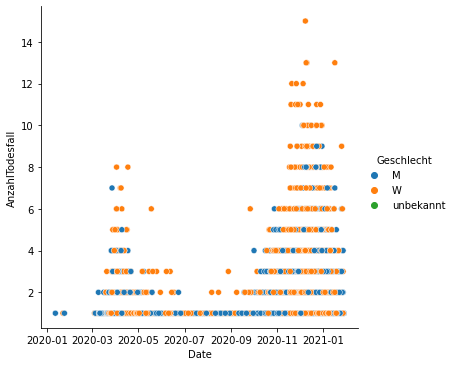
\includegraphics[scale = 0.8]{attachment/chapter_3/Scc084}
	\caption{Todesfälle}
\end{figure} 
\begin{figure}[H]
	\centering
	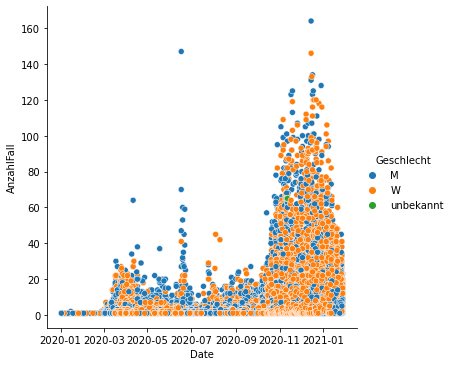
\includegraphics[scale = 0.8]{attachment/chapter_3/Scc085}
	\caption{Infektionen}
\end{figure} 
\begin{figure}[H]
	\centering
	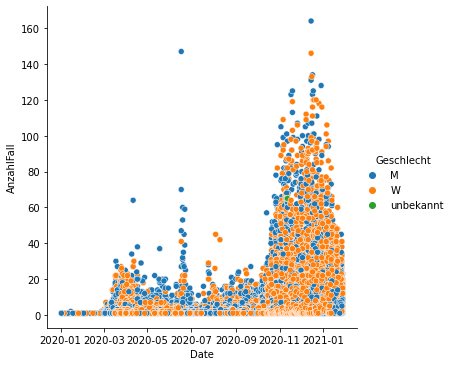
\includegraphics[scale = 0.8]{attachment/chapter_3/Scc085}
	\caption{FallAnzahl nach Altersgruppen}
\end{figure} 

\paragraph{Displot metrische Variable}
\begin{lstlisting}[style=python]
	sns.distplot(df_SKA["AnzahlFall"])
\end{lstlisting}
\begin{figure}[H]
	\centering
	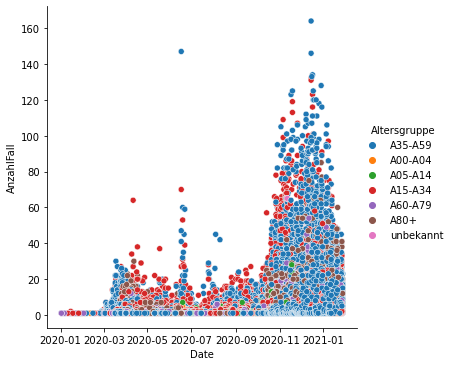
\includegraphics[scale = 0.8]{attachment/chapter_3/Scc086}
	\caption{FallAnzahl nach Altersgruppen}
\end{figure} 

Mit .replace() können die string Werte in numerische Werte überführt werden.
\begin{figure}[H]
	\centering
	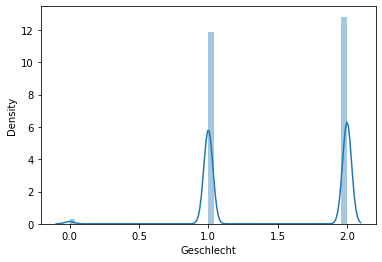
\includegraphics[scale = 0.8]{attachment/chapter_3/Scc089}
\end{figure} 

\paragraph{Boxplot}
\begin{lstlisting}[style=python]
	sns.catplot(x="AnzahlFall", kind="box", data=df_SKA)
\end{lstlisting}
\begin{figure}[H]
	\centering
	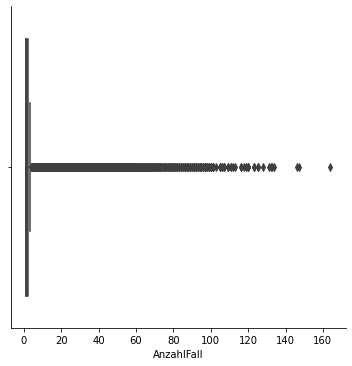
\includegraphics[scale = 0.8]{attachment/chapter_3/Scc088}
	\caption{FallAnzahl nach Altersgruppen}
\end{figure} 




\subsection{Data Visulization - Matplotlib}
\subsubsection{Preparation}
Die Daten für die Grafiken in \textit{Matplot.pyplot} bereit zu stellen, müssen einige Kriterien erfüllt sein.
\paragraph{Spalteauslesen}
Es bietet sich an, die Spalten sich als Dataframe ausgeben zu lassen. In \textit{VStudio} können diese übersichtlich angezeigt werden.
\begin{lstlisting}[style=python]
	df_i_columns = Dataframe(df_i.columns)
\end{lstlisting}
Es dürfen keine NULL Werte beinhaltet sein. Über den \textit{.info} werden die Kriterien des Dataframes ausgegeben.
\begin{lstlisting}[style=Python]
	df_i.info()
\end{lstlisting}
\begin{figure}[H]
	\centering
	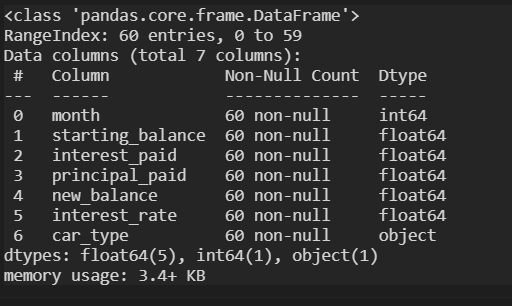
\includegraphics[scale = 0.8]{attachment/chapter_4/Scc003}
\end{figure}

\paragraph{Filter - Praxis}
Es gibt mehrere Möglichkeiten Filter bezüglich des Dataframes anzuwenden.
Eine Methode ist, Filter anzulegen und diese kombiniert über \textit{.loc} anzuwenden.
\begin{lstlisting}[style=Python]
	#%%
	# Configure Filters
	
	df_i_filter_1 = df_i[df_i_columns.iloc[8,0]] == "VW Golf R"
	df_i_filter_2 = df_i[df_i_columns.iloc[7,0]] == 0.029
	
	#%%
	# Apply one filters
	# First Methode
	df_i[df_i_filter_1]
	
	#%%
	# Apply one filters
	# First Methode
	df_filter = df_i.iloc[df_i_filter_1.array]
	df_filter.head()
	
	#%%
	# Apply two filters
	# First Methode
	df_filter_two = df_i[df_i_filter_1 & df_i_filter_2]
	df_filter_two.head()
	
	
	# %%
	# Apply two filters
	# Secound Methode
	
	df_filter_two = df_i.loc[df_i_filter_1 & df_i_filter_2]
	df_filter_two.head()
\end{lstlisting}

\paragraph{Transformation: Numpy - ndarray} 
Einzelne Spalten müssen wir die einzelne Darstellung in \textit{ndarray} umgewandelt werden. Es gibt zwei Methoden in \textit{pandas} welche dies tun. Ebenso gibt es Methoden, welche nur Arrays ausgeben, dies aber nicht in \textit{ndarrays} transformieren.
\begin{itemize}
	\item \textit{df.values} oder 
	\item \textit{df.to$\_$numpy()}
\end{itemize}
\begin{lstlisting}[style=Python]
	# %%
	### Preparation for mathplot
	
	# ndarray (numpy) Month
	varSelCol_3 = df_i_columns.iloc[0,0]
	nda_Month = df_i[varSelCol_3].values
	
	# ndarray (numpy) Interest Paid
	varSelCol_3 = df_i_columns.iloc[[0,1,2],0]
	nda_interest_paid = df_i[varSelCol_3].values
	
	# ndarray (numpy) Prinzipal Paid
	varSelCol_3 = df_i_columns.iloc[3,0]
	nda_prinzipal_paid = df_i[varSelCol_3].to_numpy()
\end{lstlisting}
\begin{figure}[H]
	\centering
	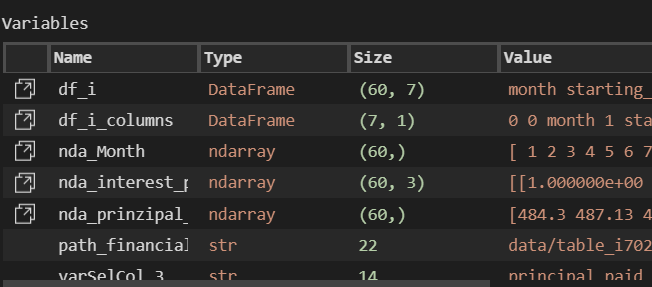
\includegraphics[scale = 0.8]{attachment/chapter_4/Scc004}
\end{figure}
Die letzte Funktion wird von \textit{pandas} vorgeschlagen, als die zu bevorzugenden Funktion. \\

Die Auslesung einer Spalte reicht nicht aus. Hierbei wird nur eine \textit{Series} zurückgegeben.

)
\paragraph{Historischer Abriss}
Um fehlende Werte in Python zu verstehen, muss die historisch, gewachsenen Struktur der Pakete \textit{pandas}, \textit{NumPy}, sowie der Sprache \gls{R} betrachtet werden.\\

\begin{itemize}
	\item Die Begriffe \gls{g_None} und \gls{g_NULL} sind inhaltlich gleich. In Python wird nur \gls{g_None} verwendet. Als Beispiel in \gls{CPP} und Power BI wird \gls{g_NULL} verwendet.
	\item In Python selbst gibt es viele Pakete (\textit{NumPy}, \textit{Math}) welche \gls{g_NaN} ermöglichen: $np.nan$.
	\item Die Pakete \textit{pandas} und \textit{NumPy} sind in Anlehnung an \gls{R} geschrieben worden.
	\item Die Begrifflichkeit \gls{Na} gibt in Python nicht, sondern wurde nur aus historischen Gründen übernommen.
	\item \textit{Pandas} ist aufbauend auf \textit{NumPy} geschrieben worden. Es unterscheidet jedoch nicht mehr zwischen NaN aus \textit{NumPy} und \gls{g_None}. Die Funktionen 
	\begin{align}
		Dataframe.isnull()\\
		Dataframe.isna()
	\end{align}
	geben das gleich aus.
\end{itemize}

\paragraph{Umgang in Pandas mit NaN}
\textit{Pandas} unterscheidet bei der Suche nach fehlenden Daten nicht zwischen den beiden Datentypen \gls{g_None} und \gls{NaN}. Die Funktionen
\begin{align}
	pandas.isnull()
\end{align}
und 
\begin{align}
	pandas.isna()
\end{align}
geben die gleichen \textit{Wahr}/\textit{Falsch} Werte zurück. Dies gilt ebenso bei der Anwendung auf Dataframes 
\begin{lstlisting}[style=Python]
	df = pd.DataFrame([2,np.nan, None])
	df["2"] = df[0].isnull()
	df["3"] = df[0].isna()
	df
\end{lstlisting}
\begin{figure}[H]
	\centering
	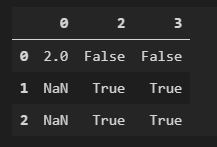
\includegraphics[scale = 0.8]{attachment/chapter_4/Scc008}
\end{figure}
Hinzu kommt, dass Pandas \gls{g_None} in \gls{NaN} in \gls{NaN} umwandelt. Die Funktion \textit{isnull()} und \textit{isna()} ist auf das Fundament in \gls{R} zurück zuführen.\\

Die Werte in Variablen abgespeichert, erzielen das gleiche Resulat, bei einer Gleichheitsabfrage:
\begin{lstlisting}[style=Python]
	x = np.nan
	y = np.nan
	x == y # False
\end{lstlisting}
Wir gefragt, ob es sich um das gleiche Objekt \bl{is} handelt, wird bei den Variablen 
\begin{lstlisting}[style=Python]
	x is y # True
\end{lstlisting}
dies bejaht. \\

Befindet sich \textit{NaN} in einem Dataframe, wird \textit{false} zurückgegeben:
\begin{lstlisting}[style=Python]
	df = pd.DataFrame([None,np.nan, 3], [4, None, None])
	df["5"] = df[0] == np.nan
	df["6"] = df[0] is np.nan
	df
\end{lstlisting}

\begin{figure}[H]
	\centering
	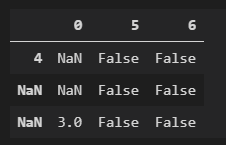
\includegraphics[scale = 0.8]{attachment/chapter_4/Scc009}
\end{figure}
Der Grund ist, dass im Dataframe \gls{g_NaN} anders codiert ist. Für weiteres siehe das Glossar: \gls{g_NaN}.

\paragraph{Umgang mit None}
Der Wert \gls{g_None} ist immer der selbe, weshalb die Gleichheitsabfrage \textit{true} zurückgibt. Ebenso ist die Identität eines jeden \gls{g_None} Wertes auf ein Objekt zurückzuführen: TypNone
\begin{lstlisting}[style=Python]
	x = None
	y = None
	x == y # True
	x is y # True
\end{lstlisting}

\paragraph{Näheres zu None und NULL}
In Python existiert das Konzept \gls{g_None}, welches aus die Funktion von \gls{g_NULL} aus anderen Sprachen übernimmt. Die Funktion \textit{print()} ist Funktion, welche \gls{g_None} wieder gibt. 
\begin{lstlisting}[style=Python]
	print("Hello")
	>>> Hello
	print(print("Hello"))
	>>> Hello
	>>> None
\end{lstlisting}

\footnote{
	\href{https://www.r-bloggers.com/2010/04/r-na-vs-null/}{Unterschied in R zwischen NaN und NULL}, \href{https://datascience.stackexchange.com/questions/37878/difference-between-isna-and-isnull-in-pandas}{Unterschied zwischen den Funktionen in Pandas und NumPy}, 
	\href{https://www.r-bloggers.com/2010/04/r-na-vs-null/}{r-na-vs-null},
	\href{https://realpython.com/null-in-python/}{Null in Python}
}

\paragraph{Removing or filling in missing data}
\paragraph{.dropna()}
\begin{lstlisting}[style=Python]
	
	### Loading Data
	#path_financial = "data/car_financing.csv"
	path_financial = "data/table_i702t60.csv"
	df = pd.read_csv(path_financial)
	
	# %% Scaning Data
	df.info()
	# %% Adding a missing value
	df.iloc[2,2] = np.nan
	# %% Check up
	df.info()
	# %% Droping rows
	'''
	The function .dropna() allows to delete any rows, with np.nan values.
	axis:[0,1], default 0
	how : ['any,all'], default 'any'
	- 'any': If any nan are present drop the row or column
	- 'all': If all values are nan, drop row or column
	etc.
	'''
	df.dropna(how='any', inplace = True)
\end{lstlisting} 
\paragraph{Fill-In: General} Im allgemeinen ist \textit{.iloc()} nicht dafür ausgelegt, dass diese Funktion Werte im ursprünglichen Dataframe anpassen. Es kann verwendet werden, wie zum Beispiel:
\begin{lstlisting}[style=Python]
	#%% Replace Values
	for i in range(3,6):
	df.iloc[i,2]= 3
\end{lstlisting}
\begin{figure}[H]
	\centering
	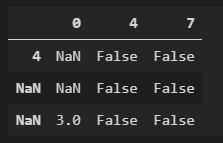
\includegraphics[scale = 0.8]{attachment/chapter_4/Scc010}
\end{figure}
Gleich ist es möglich mit der dopple Indexierung die Werte zu ändern:
\begin{lstlisting}[style=Python]
	# %% For loop Changing Value
	for i, j in enumerate(df_column):
	df.loc[i,j] = np.nan
\end{lstlisting}
Achtung, wenn Zeilen fehlen, oder durch vorherige Schritte entfernt werden, sind die Indexies nicht mehr vorhanden, und können zu Problemen führen:
\paragraph{Fill-In: fillna()} Der entsprechende Bereich kann ersetzt werden.
\begin{lstlisting}[style=Python]
	'''
	DataFrame.fillna(value=None, method=None, axis=None, inplace=False, limit=None, downcast=None)[source]
	Fill NA/NaN values using the specified method.
	
	Parameters
	valuescalar, dict, Series, or DataFrame
	Value to use to fill holes (e.g. 0), alternately a dict/Series/DataFrame of values specifying which value to use for each index (for a Series) or column (for a DataFrame). Values not in the dict/Series/DataFrame will not be filled. This value cannot be a list.
	
	method{‘backfill’, ‘bfill’, ‘pad’, ‘ffill’, None}, default None
	Method to use for filling holes in reindexed Series pad / ffill: propagate last valid observation forward to next valid backfill / bfill: use next valid observation to fill gap.
	
	axis{0 or ‘index’, 1 or ‘columns’}
	Axis along which to fill missing values.
	
	inplacebool, default False
	If True, fill in-place. Note: this will modify any other views on this object (e.g., a no-copy slice for a column in a DataFrame).
	
	limitint, default None
	If method is specified, this is the maximum number of consecutive NaN values to forward/backward fill. In other words, if there is a gap with more than this number of consecutive NaNs, it will only be partially filled. If method is not specified, this is the maximum number of entries along the entire axis where NaNs will be filled. Must be greater than 0 if not None.
	
	downcastdict, default is None
	A dict of item->dtype of what to downcast if possible, or the string ‘infer’ which will try to downcast to an appropriate equal type (e.g. float64 to int64 if possible).
	
	Returns
	DataFrame or None
	Object with missing values filled or None if inplace=True.
	'''
\end{lstlisting}
Die Funktion \textit{.fillna()} ermöglicht es \gls{NaN} Wert direkt zu ersetzten.
\begin{figure}[H]
	\centering
	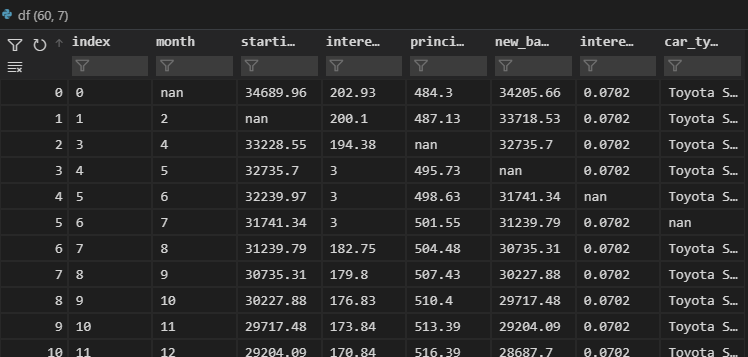
\includegraphics[scale = 0.8]{attachment/chapter_4/Scc012}
\end{figure}
\begin{lstlisting}[style=Python]
	df.info()
\end{lstlisting}
\begin{figure}[H]
	\centering
	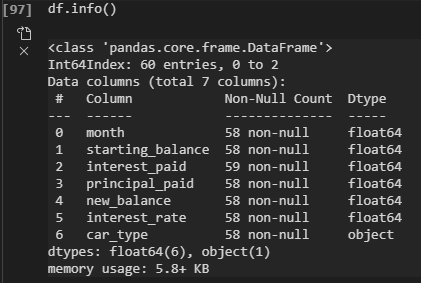
\includegraphics[scale = 0.8]{attachment/chapter_4/Scc013}
\end{figure}
\begin{lstlisting}[style=Python]
	df.fillna("x", inplace = True)
\end{lstlisting}
\begin{lstlisting}[style=Python]
	df.info()
\end{lstlisting}
\begin{figure}[H]
	\centering
	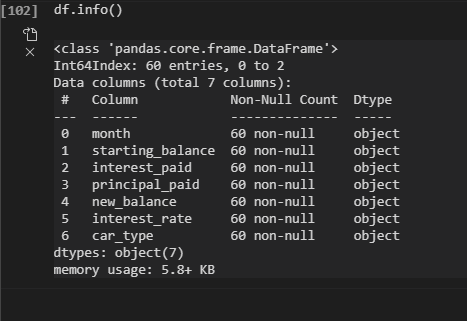
\includegraphics[scale = 0.8]{attachment/chapter_4/Scc014}
\end{figure}

\paragraph{Fill in directly}
\begin{lstlisting}[style=Python]
	varIsNull = df["interest_paid"].isna()
	df["interest_paid"].iloc[varIsNull] = "y"
\end{lstlisting}

\paragraph{Converting Dataframe to NumPy}\label{Converting Dataframe to NumP}

\begin{lstlisting}[style=Python]
	df.to_numpy() # NumPy Array
	df.values # NumPy Array
	df.to_dict() # Dictionaries
\end{lstlisting}
\subsubsection{Simple Plot}
Die Funktion \textit{plt.plot()} benötigt als Inputs \textbf{NumPy Arrays}. Liegt Datensätze in Form eines pandas Dataframe vor, so müssen die einzelnen Spalten in solche konvertiert werden, siehe \ref{Converting Dataframe to NumP}.

\begin{lstlisting}[style=Python]
	#%% Import Packages & Data
	
	import pandas as pd
	import numpy as np
	import matplotlib.pyplot as plt 
	import seaborn as sns 
	
	
	'''Loading Data'''
	path_financial = "data/car_financing.csv"
	#path_financial = "data/table_i702t60.csv"
	df_i = pd.read_csv(path_financial)
	
	''' Extract column names'''
	df_i_columns = pd.DataFrame(df_i.columns)
	
	#%% Check for NaN or Null Values
	df_i["car_type"].unique()
	
	# %% Filter with iloc
	filter_cartype = df_i["car_type"] == "Toyota Corolla"
	df_i = df_i.iloc[filter_cartype.array]
	
	
	# %% Preparation for mathplot
	
	'''Month'''
	varSelCol_3 = df_i_columns.iloc[0,0]
	nda_Month = df_i[varSelCol_3].to_numpy()
	
	''' Interest Paid'''
	varSelCol_3 = df_i_columns.iloc[3,0]
	nda_interest_paid = df_i[varSelCol_3].values
	
	'''Prinzipal Paid'''
	varSelCol_3 = df_i_columns.iloc[4,0]
	nda_prinzipal_paid = df_i[varSelCol_3].to_numpy()
\end{lstlisting}
Ist dies geschehen, kann mit \textit{plt.plot()} ein Graf erzeugt werden.

\begin{lstlisting}[style=Python]
	plt.plot(nda_Month,nda_interest_paid)
\end{lstlisting}

\begin{figure}[H]
	\centering
	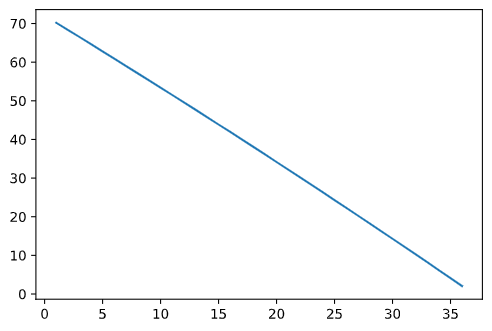
\includegraphics[scale = 0.8]{attachment/chapter_4/Scc015}
\end{figure}

Wird zwei \textit{plt.plot()} erstellt, werden diese in einer Grafik zusammengefügt
\begin{lstlisting}[style=Python]
	# %% Plot two graphs in one grahic
	plt.plot(nda_Month, nda_prinzipal_paid)
	plt.plot(nda_Month, nda_interest_paid)
\end{lstlisting}
\begin{figure}[H]
	\centering
	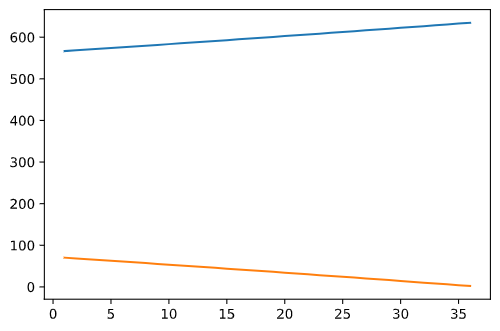
\includegraphics[scale = 0.8]{attachment/chapter_4/Scc016}
\end{figure}
\paragraph{Styles}
Mit \textit{plt.style.available} werden die verschiedensten Styles in Matplot angezeigt. Unter Einbindung von seaborn stehen mehr Styles zur Verfügung.
\begin{lstlisting}[style=Python]
	# %% Chosoe Style
	plt.style.available
\end{lstlisting}
\begin{figure}[H]
	\centering
	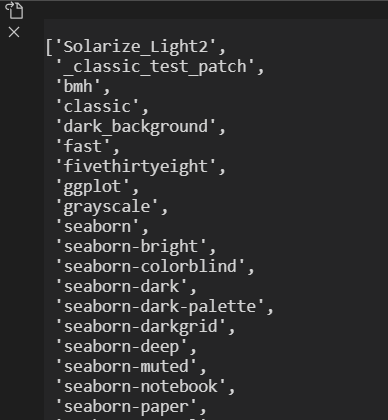
\includegraphics[scale = 0.8]{attachment/chapter_4/Scc017}
\end{figure}
Den Style zu ändern, erfolgt über \textit{plt.style.use()}.
\begin{lstlisting}[style=Python]
	# %% Choose Style
	plt.style.use("seaborn-dark")
	plt.plot(nda_Month, nda_prinzipal_paid)
\end{lstlisting}

\paragraph{Marker Type and Colors}
\begin{itemize}
	\item maker - Einzelne Datenpunkte
	\item markersize - Größe von Marker
	\item c - Colour Template
\end{itemize}
\begin{lstlisting}[style=Python]
	# %% Marker and Colour
	Grafik_1 = plt.plot(nda_Month, nda_prinzipal_paid, marker = ".", markersize = 10, c = "k")
	Grafik_2 = plt.plot(nda_Month, nda_interest_paid, marker = ".", markersize = 8, c = "k")
\end{lstlisting}
\begin{figure}[H]
	\centering
	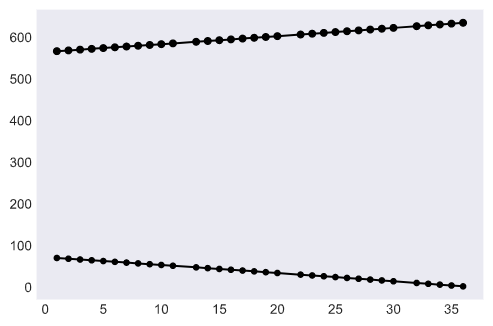
\includegraphics[scale = 0.8]{attachment/chapter_4/Scc018}
\end{figure}




\subsubsection{MATLAB-Style vs Object-Oriented Style}
\paragraph{Subplots - Two simple Figures}
Über Matplotlib können zwei verschiedene Syntaxen verwendet werden:
\begin{itemize}
	\item \textbf{MATLAB} Style und oder
	\item \textbf{Objektorientierte} Syntax. \footnote{\cite{URL.Python-Tutorial}, \cite{}Book.Python-DSci}
\end{itemize}

Die Syntax wurde von MATLAB übernommen, weshalb es viele Gleichheiten mit der Python Alternative, Matplotlib, gibt.\\

\paragraph{Matlab}
Im ersten Beispiel wird dargestellt, wie in dem \textit{MATLAB-Style} Grafiken mit Hilfe von \textit{plt.subplot()} dargestellt werden.\footnote{Wird \textit{plt.subplot() ohne Argument erstellt, so wird eine Objekt mit einer Zeile und einer Spalte erstellt.}}
\begin{itemize}
	\item Die Parameter \textit{nrows}, \textit{ncols} und \textit{index} der Funktion \textit{subplot()} geben an, wie viele Panele erstellt werden.
	\item Dabei wird für jeden Subplot die gleich Konfiguration benötigt. Der \textit{index} gibt dabei an, in welchem Panal der Plot angefügt werden soll.
	\item Wird \textit{plt.figure} nicht angegeben, wird bei dieses \textit{plt.subplot} impliziert erstellt
\end{itemize}

\begin{lstlisting}[style=Python]
	#%% Import Packages
	import pandas as pd
	import numpy as np
	import matplotlib.pyplot as plt 
	import seaborn as sns 
	
	#%% Creating Variables
	x = np.linspace(0,50,1000)
	
	#%% Create a plot figure
	plt.figure() # create a figure object
	
	plt.subplot(2,2,1) # row, column, panel
	plt.plot(x, np.sin(x))
	
	plt.subplot(2,2,4)
	plt.plot(x, np.cos(x))
	
	plt.subplot(2,2,2)
	plt.plot(x, np.sin(x)+2)
	
	plt.subplot(2,2,3)
	plt.plot(x, np.sin(x)*3)
	
	plt.title("Hello") # Title for the figure
\end{lstlisting} \footnote{\cite[240]{Book.Python-DSci}}





Der Nachteil dieses Styles ist es, dass es aufwendig ist, neue Panale hinzuzufügen. Es müssen alle Konfigurationen angepasst werden.\\
\begin{figure}[H]
	\centering
	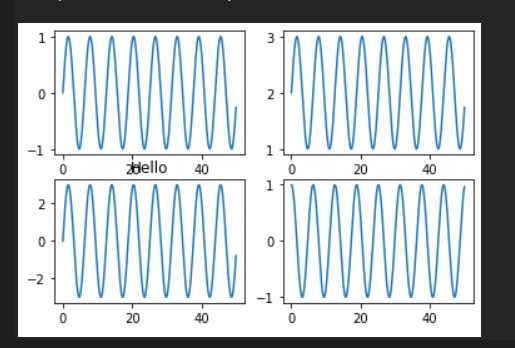
\includegraphics[scale = 0.8]{attachment/chapter_4/Scc019}
\end{figure}
\paragraph{OO}
In dem objekt-orientierenden Style wird eine Figure Objekt erstellt und die Panele in dem Objekt \textbf{ax} gespeichert. Die Anzahl der Panele bestimmt die Anzahl der geplotteten Grafiken. \\

\textbf{ACHTUNG:} Die Funktion heißt plt.subplot\textcolor{red}{s} nicht plt.subplot.

\begin{lstlisting}[style=Python]
	fig, ax = plt.subplots(2)
	
	ax[0].plot(x, np.sin(x))
	ax[1].plot(x, np.sin(-x))
\end{lstlisting}
\begin{figure}[H]
	\centering
	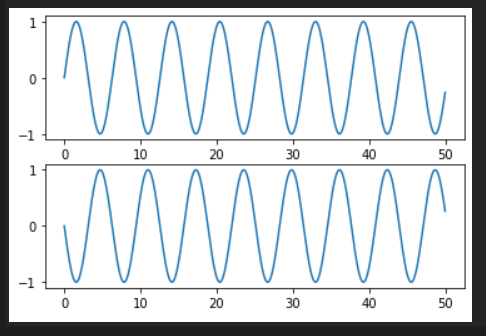
\includegraphics[scale = 0.8]{attachment/chapter_4/Scc020}
\end{figure}

\paragraph{Simple Linie Plot}
Die Instanzen der Objekte Figure und Axes sehen wie folgt leer aus.
\begin{lstlisting}[style=Python]
	# %% Seaboarn Style
	plt.style.use('seaborn-whitegrid')
	
	figure_l = plt.figure() # Create instance of the object figure
	axis_l = plt.axes() # Create instance of the object axes
\end{lstlisting}
\begin{figure}[H]
	\centering
	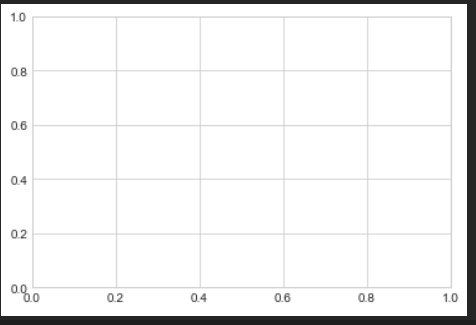
\includegraphics[scale = 0.8]{attachment/chapter_4/Scc021}
\end{figure}
Dabei produziert der Befehlt ohne \textit{plt.figure} eine Grafik, hingegen anders herum nicht.

Die Instanz \textit{Figure} kann so verstanden werden, dass es alle Instanzen von \textit{axis}, \textit{label}, \textit{title} und \textit{graphics} umschließt.

Im Folgenden soll die Funktion $f(x)=\sin(x)$ mit $x\in [0,10]$ in den zwei Formen abgebildet werden. Im objekt-orientierten Style wird dies über die Objekte Axis und Figure dargestellt:
\begin{lstlisting}[style=python]
	# %% Seaboarn Style
	plt.style.use('seaborn-whitegrid')
	
	x_sin = np.linspace(0,5,num=1000) # Generate Input
	
	figure_l = plt.figure() # Create instance of the object figure
	axis_l = plt.axes() # Create instance of the object axes
	
	axis_l.plot(x, np.sin(x))
\end{lstlisting}
Ohne dies kann es über 
\begin{lstlisting}[style=python]
	plt.plot(x,np.sin(x))
\end{lstlisting}
angesteuert werden.

\paragraph{Same Function in Both Styles}
Der Prefix lautet \textit{plt.} oder \textit{ax.}
\begin{itemize}
	\item legend()
	\item plot()
	\item etc.
\end{itemize}

\paragraph{Different Function in Both Styles}
Es gibt Funktionen, die den gleichen Inhalt vermitteln, aber unterschiedlich Syntax besitzen.
\begin{itemize}
	\item Achsen Grenze bestimmen:
	\begin{lstlisting}[style=python]
		# M
		plt.plot()
		plt.xlim()
		# OO
		ax.plot()
		ax.set_xlim()
	\end{lstlisting}
	\item Achsen Titel bestimmen:
	\begin{lstlisting}[style=python]
		# M
		plt.plot()
		plt.xlabel()
		# OO
		ax.plot()
		ax.set_xlabel())
	\end{lstlisting}
	\item Grafik Titel bestimmen:
	\begin{lstlisting}[style=python]
		# M
		plt.plot()
		plt.titel()
		# OO
		ax.plot()
		ax.set_title())
	\end{lstlisting}
\end{itemize}
Der Vorteil gegenüber de Matlab-Notierung ist, dass über die \textit{.set()} Funktion die einzelnen Bestanteile gemeinsam aufgerufen werden können.
\begin{lstlisting}[style=python]
	
	# %% Seaboarn Style
	plt.style.use('seaborn-whitegrid')
	
	x_sin = np.linspace(0,5,num=1000) # Generate Input
	
	figure_l = plt.figure() # Create instance of the object figure
	axis_l = plt.axes() # Create instance of the object axes
	
	axis_l.plot(x, np.sin(x))
	
	axis_l.set(xlim=(0,10), ylim=(-1,1), title="Cool")
\end{lstlisting}

\begin{figure}[H]
	\centering
	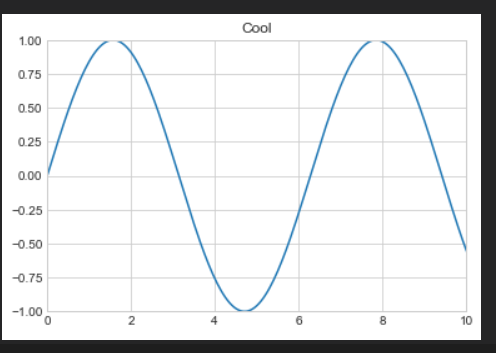
\includegraphics[scale = 0.8]{attachment/chapter_4/Scc022}
\end{figure}

